% Compelling argument demonstrating success criteria met, or well-justified explanation of different direction taken.

% Excellent critical thought and interpretation which substantiate any claims of success.

\label{sec:4}

\section{Review of Success Criteria}
\label{sec:review-of-success-criteria}
My project has met all success criteria as outlined below:

\begin{enumerate}[font=\bfseries]
    \item[1a.]\textbf{Multiple agents will be able to localize themselves within a world using purely visual data.} \\
    My system is the first decentralized SLAM system capable of operating using only monocular camera data. This removes the need for large and expensive stereo camera, LiDAR or RGBD sensors.

    \item[1b.]\textbf{Agents will be capable of communicating with each other to build a shared understanding of the world.} \\
    Agents use ROS to perform decentralized and reliable communication with eachother, and are able to merge maps and share key frames to build a shared world.

    \item[1c.]\textbf{Agents will be able to act independently, failing gracefully if it loses communication with its peers.} \\
    Agents fall back to performing single-agent visual SLAM when communication with their peers is degraded or lost. Once communication is regained, the agents share their unsent map data.

    \item[2.]\textbf{Evaluate the capabilities of the system compared to a comparable single-agent system.} \\
    This is performed in the \nameref{sec:benchmarking} section. I go beyond the original success criteria by also comparing my system to comparable multi-agent systems, demonstrating my system's superior performance.

\end{enumerate}


After discussions with my supervisor, we decided to not pursue my original project extensions of optimizing data transfer rates and adding additional sensors inputs to the system. We instead chose to focus on deploying the SLAM system on physical robots and building infrastructure around the system to improve usability and benifit the wider open source community.

Deploying my system on real robots was a considerable amount of work, however I beleive it was important as it provides evidence of the real world usability of my system and how my sofware engineering decisions has allowed it to easily be deployed to real robots. Additionaly it demonstrates my system working in a real distributed system as opposed to simuluations on a single device.

\section{Benchmarking}
\label{sec:benchmarking}
This section will benchmark the performance of my system when run on industry standard visual SLAM datasets. All evaluations are run using only monocular camera data.

The Central Management Interface is used to stream the dataset to the agents and my library \textit{Multi Agent EVO} is used to provide the Absolute Trajectory Error (ATE).

\subsection{EuRoC Machine Hall}
\label{sec:euroc-machine-hall}
The EuRoC Machine Hall dataset \autocite{burri2016euroc} is one of the most widely used visual SLAM datasets, providing a 752x480 20fps video feed and millimeter level ground truth data at 20hz. The camera rig is attached to a Micro Aerial Vehicle (MAV) which flies through a machine room approxamately 15x15 meters in size. To simulate a multi-agent dataset, we run the Machine Hall 01-03 scenarios in parallel on three agents.

% All three agents merge initialize maps of vastly different scales but are able to merge within TODO seconds and begin sharing map data.

\autoref{fig:euroc-mh-01-03-5-trials} presents the RMS absolute trajectory error and total system data transfer of my distributed system running this dataset. The median RMS ATE is 5.9cm over the 279 meter total trajectory length, demonstrating my system's very impressive accuracy. There ATEs and data transfer rates have a 1.4cm and 0.11 MB/s spread around the median respectively across 5 trials, demonstrating the repeatability and robustness of my system.

\begin{figure}[h]
    \centering
    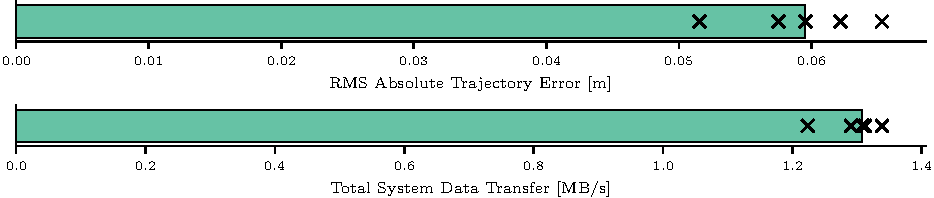
\includegraphics[width=\linewidth]{figures/comparison_apr11_mh_trajectory_b.pdf}

    \caption{Plot the RMS ATE and Total Data Transfer rate of running the EuRoC Machine Hall 01-03 dataset 5 times on my system.}
    \label{fig:euroc-mh-01-03-5-trials}
\end{figure}

To further analyze the characteristics of my SLAM system, we focus on an individual trial. \autoref{fig:euroc-traj} displays the full trajectory of the three agents compared to the ground truth, demonstrating my systems high global accuracy and relative positioning. \autoref{fig:euroc-mh-01-03-line-plot} plots the ATE as the trial progresses. It is clear that my system is performing SLAM as opposed to simple visual odometry as the ATE returns back to the baseline at the end of the trial when the agents return back to their starting position.

\begin{figure}[h]
    \centering
    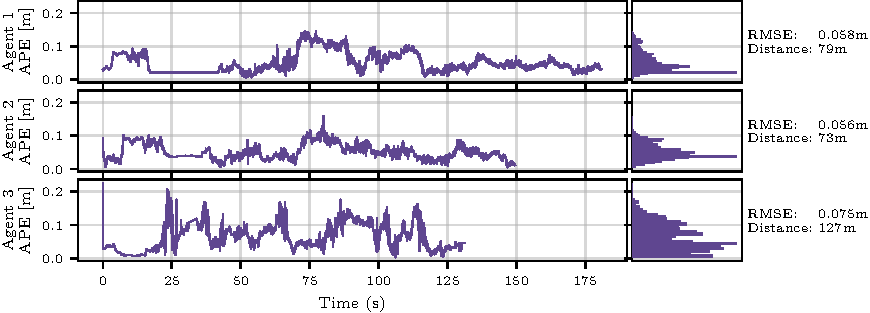
\includegraphics[width=\linewidth]{figures/EuRoC_MH_01-03_line_plot.pdf}

    \caption{Plot of my system's absolute trajectory error (ATE) with respect to the ground truth when running the EuRoC Machine Hall 01-03 scenarios in parallel on three agents.\captionbreak RMSE represents the root mean square of the ATE.}
    \label{fig:euroc-mh-01-03-line-plot}
\end{figure}

We now analyze the network usage presented in \autoref{fig:euroc-mh-01-02-bandwith}. Initially, the agents send bag of word information before quickly detecing a merge opportunity. Agent 1 procedes to send its full map to agent 2, which can be seen in the large initial spike in network bandwith. The agents successfully merge, and begin exchanging key frames. The rate of key frame data being sent rises and falls depending on how much new area the agent is exploring.

Along with sending key frames, the agents sporadically send map points to refine their map alignment. This occurs less frequently the longer system runs due to the additive increase multiplicative decrease method used to schedule map alignments, described in the \nameref{sec:map-alignment-refiner} section. However, the size of the messages also grows over time due to the larger number of tracked map points.

The data exchanged between agents largely consists of new key frames, and further work should be dedicated to optimizing the serialized representation of key frames.

\begin{figure}[h]
    \centering
    \begin{subfigure}[b]{0.55\linewidth}
        \centering
        \marginbox{0 0 0 0} {
            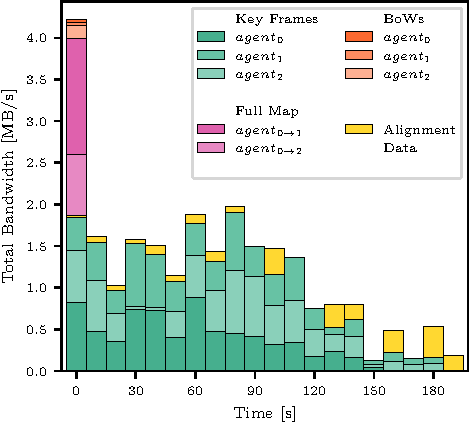
\includegraphics[width=\linewidth, valign=t]{figures/apr11_mh_trajectory_b_bandwith.pdf}
        }
        \caption{Total system data over time, segregated by message type}
    \end{subfigure}%
    ~
    \begin{subfigure}[b]{0.45\linewidth}
        \flushright
        \adjustbox{valign=t, width=\linewidth}{
            \marginbox{0.2in 0 0 0} {

                \def\arraystretch{1.2}
                \begin{tabular}{ |c|l|r|r| }
                    \cline{3-4}
                    \multicolumn{2}{}{}                       & \multicolumn{1}{|c|}{KB} & \multicolumn{1}{|c|}{Avg. KB/s}         \\
                    \hline
                    \multirow{3}{*}{Key Frames}               & $agent_0$                & 69,971                          & 351.9 \\
                                                              & $agent_1$                & 63,908                          & 321.4 \\
                                                              & $agent_2$                & 65,164                          & 327.7 \\
                    \hline
                    \multirow{3}{*}{BoWs}                     & $agent_0$                & 371                             & 1.9   \\
                                                              & $agent_1$                & 437                             & 2.2   \\
                                                              & $agent_2$                & 1,496                           & 7.5   \\
                    \hline
                    \multirow{2}{*}{Full Map}
                                                              & $agent_{0\to1}$          & 13,953                          & 70.2  \\
                                                              & $agent_{0\to2}$          & 7,319                           & 36.8  \\
                    \hline
                    \multicolumn{2}{|c|}{Alignment Data}      & 22,560                   & 113.6                                   \\
                    \hline
                    \multicolumn{2}{|c|}{\textbf{Total Data}} & \textbf{245,218}         & \textbf{1,233.1}                        \\
                    \hline
                \end{tabular}
            }
        }
        \caption{Total system data by message type}
        \vfill

        \adjustbox{valign=b, width=\linewidth}{
            \marginbox{0.2in 0 0 0.3in} {
                \def\arraystretch{1.2}
                \begin{tabular}{ |l|r|r|r|r| }
                    \cline{2-5}
                    \multicolumn{1}{}{} & \multicolumn{2}{|c|}{Sent} & \multicolumn{2}{|c|}{Received}                                                               \\
                    \cline{2-5}
                    \multicolumn{1}{}{} & \multicolumn{1}{|c|}{KB}   & \multicolumn{1}{|c|}{Avg. KB/s} & \multicolumn{1}{|c|}{KB} & \multicolumn{1}{|c|}{Avg. KB/s} \\
                    \hline
                    $agent_0$           & \textbf{114,585}           & \textbf{576.2}                  & \textbf{131,005}         & \textbf{658.8}                  \\
                    \hline
                    $agent_1$           & \textbf{64,345}            & \textbf{323.6}                  & \textbf{173,554}         & \textbf{872.8}                  \\
                    \hline
                    $agent_2$           & \textbf{66,660}            & \textbf{335.2}                  & \textbf{164,606}         & \textbf{827.7}                  \\
                    \hline
                \end{tabular}
            }
        }
        \caption{Data by agent}
    \end{subfigure}%

    \caption{Bandwidth used by the EuRoC Machine Hall 01-03 scenarios running on my SLAM system.}
    \label{fig:euroc-mh-01-02-bandwith}
\end{figure}

\begin{figure}[h]
    \centering
    \captionsetup{format=plain}
    \begin{minipage}{0.45\linewidth}
        \centering
        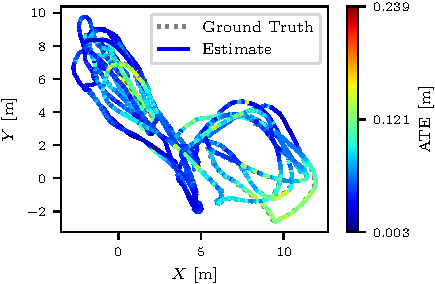
\includegraphics[height=2.2in]{figures/apr11_mh_trajectory_b_trajectory.pdf}
        \caption{EuRoC Machine Hall 01-03 estimated trajectory and ground truth.}
        \label{fig:euroc-traj}
    \end{minipage}\hfill%
    ~
    \begin{minipage}{0.45\linewidth}
        \centering
        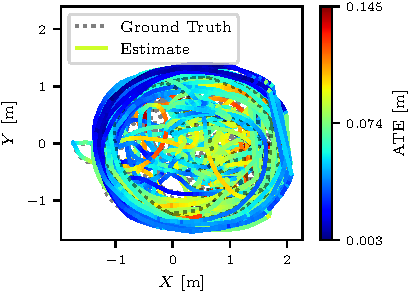
\includegraphics[height=2.2in]{figures/apr11_tum_room_trajectory_a_trajectory.pdf}
        \caption{TUM-VI Rooms 01-03 estimated trajectory and ground truth.}
        \label{fig:tum-traj}
    \end{minipage}
\end{figure}

\subsection{TUM-VI Rooms}
\label{sec:tum-rooms}
The TUM visual-intertial dataset \autocite{8593419} consists of handheld fisheye 512x512 video with ground truth data. As before, we use only monocular visual data and combine the room1-3 sessions to simulate a multi-agent dataset. The "room" environment is used for this evaluation, which is a 3x3 meter motion capture lab with plain flat walls with some posters hung up. There is less texture in this environment than the machine hall, making visual-only SLAM more difficult. As seen in the full trajectory estimate given in \autoref{fig:tum-traj}, parts of the room are revisited dozens of times by different agents, allowing us to evaluate our system's ability to relocalize agents within previously mapped environments.

\autoref{fig:tum-room-01-03-5-trials} shows that the RMS ATE is very tightly clustered around the median of 6.95cm, with one outlier caused by an agent in that trial having a slightly unoptimal map merge. The tight clustering is most likely due to the small environment with areas being revisited many times, allowing the shared map to converge on a very similar solution each time. The lower median data transfer rate of 0.84 MB/s is also due to the small environment, resulting in the agents having to share less information.

\begin{figure}[h]
    \centering
    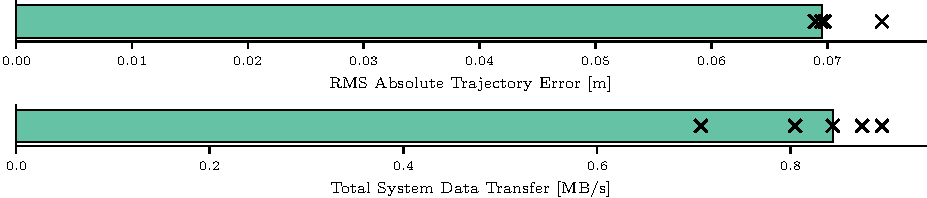
\includegraphics[width=\linewidth]{figures/comparison_apr11_tum_room_trajectory_a.pdf}

    \caption{Plot the RMS ATE and Total Data Transfer rate of running the EuRoC Machine Hall 01-03 dataset 5 times on my system.}
    \label{fig:tum-room-01-03-5-trials}
\end{figure}

Once again, we focus on an individual trial to further evaluate my system. \autoref{fig:tum-room-01-03-line-plot} shows that there is no long term error build up, demonstrating that my system is successfully localizing agents within the shared map and performing long-term map point association.

\begin{figure}[h]
    \centering
    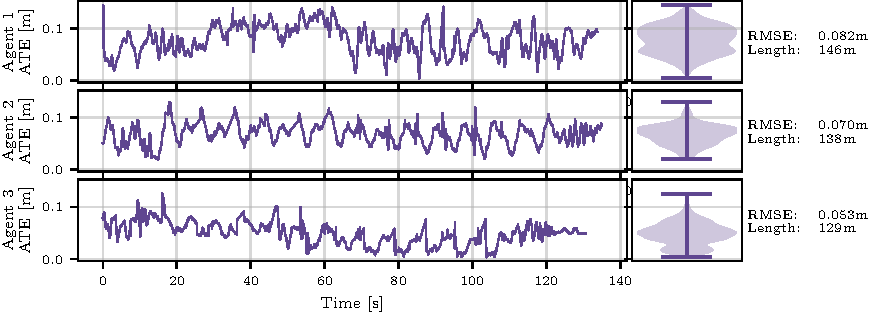
\includegraphics[width=\linewidth]{figures/apr11_tum_room_trajectory_a_line_plot.pdf}

    \caption{Plot of my system's average trajectory error (ATE) with respect to the ground truth when running the EuRoC Machine Hall 01-03 scenarios in parallel on three agents. The average RMSE of the multi-agent system is 0.062m over the 279m total trajectory length. \captionbreak RMSE represents the root mean square of the ATE.}
    \label{fig:tum-room-01-03-line-plot}
\end{figure}

\autoref{fig:tum-rooms-01-03-bandwith} presents the data transfer breakdown of a single trial, and yields similar conclusions to that of the EuRoC Machine Hall dataset. The only difference to note is the smaller key frame and alignemnt data transfer rate due to the smaller environment.

\begin{figure}[h]
    \centering
    \begin{subfigure}[b]{0.55\linewidth}
        \centering
        \marginbox{0 0 0 0} {
            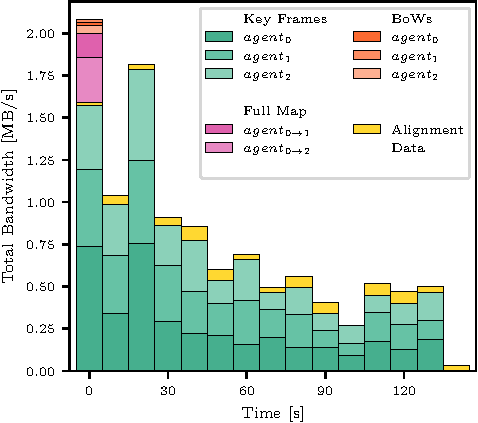
\includegraphics[width=\linewidth, valign=t]{figures/apr11_tum_room_trajectory_a_bandwith.pdf}
        }
        \caption{Total system data over time}
    \end{subfigure}%
    ~
    \begin{subfigure}[b]{0.45\linewidth}
        \flushright
        \adjustbox{valign=t, width=\linewidth}{
            \marginbox{0.2in 0 0 0} {

                \def\arraystretch{1.2}
                \begin{tabular}{ |c|l|r|r| }
                    \cline{3-4}
                    \multicolumn{2}{}{}                       & \multicolumn{1}{|c|}{KB} & \multicolumn{1}{|c|}{Avg. KB/s}         \\
                    \hline
                    \multirow{3}{*}{Key Frames}               & $agent_0$                & 37,599                          & 264.9 \\
                                                              & $agent_1$                & 33,066                          & 233.0 \\
                                                              & $agent_2$                & 29,963                          & 211.1 \\
                    \hline
                    \multirow{3}{*}{BoWs}                     & $agent_0$                & 217                             & 1.5   \\
                                                              & $agent_1$                & 188                             & 1.3   \\
                                                              & $agent_2$                & 426                             & 3.0   \\
                    \hline
                    \multirow{2}{*}{Full Map}
                                                              & $agent_{0\to1}$          & 1,472                           & 10.4  \\
                                                              & $agent_{0\to2}$          & 2,631                           & 18.5  \\
                    \hline
                    \multicolumn{2}{|c|}{Alignment Data}      & 6,947                    & 49.0                                    \\
                    \hline
                    \multicolumn{2}{|c|}{\textbf{Total Data}} & \textbf{112,511}         & \textbf{792.8}                          \\
                    \hline
                \end{tabular}
            }
        }
        \caption{Total system data by message type, segregated by message type}
        \vfill

        \adjustbox{valign=b, width=\linewidth}{
            \marginbox{0.2in 0 0 0.3in} {
                \def\arraystretch{1.2}
                \begin{tabular}{ |l|r|r|r|r| }
                    \cline{2-5}
                    \multicolumn{1}{}{} & \multicolumn{2}{|c|}{Sent} & \multicolumn{2}{|c|}{Received}                                                               \\
                    \cline{2-5}
                    \multicolumn{1}{}{} & \multicolumn{1}{|c|}{KB}   & \multicolumn{1}{|c|}{Avg. KB/s} & \multicolumn{1}{|c|}{KB} & \multicolumn{1}{|c|}{Avg. KB/s} \\
                    \hline
                    $agent_0$           & \textbf{49,083}            & \textbf{345.9}                  & \textbf{63,644}          & \textbf{448.5}                  \\
                    \hline
                    $agent_1$           & \textbf{33,254}            & \textbf{234.3}                  & \textbf{76,624}          & \textbf{539.9}                  \\
                    \hline
                    $agent_2$           & \textbf{30,389}            & \textbf{214.1}                  & \textbf{80,649}          & \textbf{568.3}                  \\
                    \hline
                \end{tabular}
            }
        }
        \caption{Data by agent}
    \end{subfigure}%

    \caption{Bandwidth used by the TUM-VI Rooms 01-03 scenarios running on my SLAM system.}
    \label{fig:tum-rooms-01-03-bandwith}
\end{figure}

%evaluate how

\section{Comparison to Related Work}
\label{sec:comparison-to-related-work}

As discussed in the \nameref{sec:relevant-work} section, my system is the first decentralized monocular vision SLAM system avaiable. This makes direct comparisons with other multi-agent SLAM systems difficult, as they rely on more accurate but bulky sensors such as stero cameras and LiDAR. However, this section still attempts to compare my system to the latest research in the field to give context to its performance relative to other state of the art systems.

We are only able to compare results using the EuRoC dataset as it is the only public dataset evaluated by CCM-SLAM. Ideally, I would run more datasets on CCM-SLAM system, however I encountered many issues when trying to build the codebase published alongside their paper. This reinforces the well known reproducibility issues within the field of visual SLAM \autocite{DBLP:journals/corr/abs-2108-01654}, which I have attempted to mitigate in my own project by publishing pre-compiled docker containers alongside my code. \textbf{My SLAM system is not specifically tweaked to perform well in the EuRoC dataset and we get similarly low RMS ATE values in both the TUM Rooms dataset and real world evaluations.}

\subsection{CCM-SLAM}
\label{sec:ccm-slam}
Centralized Collaborative Moncular SLAM (CCM-SLAM) (2019) from the ETH Zurich Vision for Robotics Lab \autocite{schmuck2019ccm} is the most comparable multi-agent SLAM system in recent literature, and is well cited in the field. Their approach also uses purely monocular vision with ORB-SLAM to the front-end tracking and local mapping stages of the SLAM pipeline, with a custom backend to integrate data from multiple agents into the shared map. To my knowledge, it is the most recent monocular vision capable multi-agent SLAM system.

The results of CCM-SLAM and my system running the EuRoC Machine Hall 01-03 dataset are presented in \autoref{fig:comparison-to-multi-agent-systems}. \textbf{It is important to note that CCM-SLAM is a centralized system, significantly simplifying their multi-agent SLAM problem compared to my distributed system.} Nevertheless, my system is able to outperform CCM-SLAM in terms of RMS ATE, demonstrating its compeditiveness. My system's total data transfered is 32\% higher than CCM-SLAM, however this could easily be reduced as I have made no attempt to optimize the data transfer efficiency of my system.

\subsection{VINS-Mono Multisession SLAM}
VINS-Mono (2018) \autocite{8421746} is a popular open source single-agent monocular vision SLAM system. While it is a multi-agent system, it has multisession capabilities. This allows multiple datasets to be played consecutively, with each session building upon the map built by the previous sessions (eg. session 2 is initialized in the map generated after running session 1). This is an easier problem than multi-agent SLAM, where the sessions are run in parallel and the agents have to share their maps in real time. As presented in \autoref{fig:comparison-to-multi-agent-systems}, my system still outperforms VINS-Mono multisession.

\begin{figure}[h]
    \centering
    \def\arraystretch{1.2}
    \begin{tabular}{ |l|l|l|l| }
        \cline{2-4}
        \multicolumn{1}{c|}{} & My system      & CCM-SLAM$^1$ & VINS-Mono$^2$ \\
        \hline
        RMS ATE [m]$^3$       & \textbf{0.059} & 0.077        & 0.074         \\
        \hline
        % Data Transfer [MB/s]  & 1.31               & \textbf{0.99}     & N/A                \\
        % \hline
    \end{tabular}

    \caption{Comparison of my SLAM system to comparable state of the art multi-agent systems running the EuRoC Machine Hall 01-03 dataset with only monocular images. \captionbreak $^1$CCM-SLAM is a centralized system, as opposed to my decentralized system. \\ $^2$VINS-Mono is a single-agent SLAM system run in multisession mode. \\ $^3$RMS ATE is taken as the median of 5 trials. Results of external systems are taken from \autocite{schmuck2019ccm}.}
    \label{fig:comparison-to-multi-agent-systems}
\end{figure}

\subsection{Comparison to Single-Agent SLAM Systems}
Along with providing relative positioning, we would hypothesise a multi-agent SLAM system to have higher accuracy than a comparable single-agent system. However, the reality is far more complex than this simple assumption. \autoref{fig:comparison-to-single-agent-systems} presents my multi-agent system's errors compared to ORB-SLAM3 running the datasets individually. ORB-SLAM3 is used to perform the tracking and local mapping in my multi-agent system, and is widely regarded as the most accurate single-agent SLAM system currently avaiable so there is no suprise that it performs very well.

An observation is that some dataset sessions have only a marginal improvment in error over the single-agent system, which I hypothesize is the result of the varying ability amoung agents to utilize the shared map. For example, the TUM-VI Room dataset has very similar performance in both the single-agent and multi-agent systems since the environment is very small and areas of the map are revisited dozens of times in one session. This reduces the benefit of a multi-agent system's as a single-agent system already observes more than enough data to build an accurate map of the world, making the extra data provided by the additional agents in a multi-agent system redundant.

TODO talk about euroc dataset

\begin{figure}[h]
    \centering
    \def\arraystretch{1.2}
    \begin{tabular}{ |l|l|l| }
        \cline{2-3}
        \multicolumn{1}{c|}{} & My system$^1$  & ORB-SLAM3$^2$  \\
        \hline
        EuRoC MH 01           & 0.051          & \textbf{0.049} \\
        EuRoC MH 02           & \textbf{0.048} & 0.099          \\
        EuRoC MH 03           & \textbf{0.058} & 0.062          \\
        \hline
        TUM-VI Room 1         & 0.072          & \textbf{0.071} \\
        TUM-VI Room 2         & \textbf{0.048} & 0.050          \\
        TUM-VI Room 3         & \textbf{0.041} & 0.042          \\
        \hline
        % Data Transfer [MB/s]  & 1.31               & \textbf{0.99}     & N/A                \\
        % \hline
    \end{tabular}

    \caption{Comparison of individual agent errors from my multi-agent SLAM system and the single-agent ORB-SLAM system. All results are the median of 5 runs. \captionbreak $^1$Trajectories are aligned with the ground truth on a per-agent basis so we can compare each individual agent's performance in isolation. \\ $^2$Results are generated by running ORB-SLAM3 on my device with its default settings for the EuRoC dataset.}
    \label{fig:comparison-to-single-agent-systems}
\end{figure}

On a broader note, many researchers believe single-agent SLAM to be a solved problem. This is reflected by the results seen here, where single-agent systems are able to give incredibly low trajectory errors that even multi-agent systems with far more data struggle to improve upon. This is not something specific to my system – many other multi-agent systems do not have significantly higher accuracies than single-agent systems.

Therefore, I believe that the primary benifits of a multi-agent system are its ability to provide relative positioning for path planning and collision avoidance capabilities, and to build a shared map of the environment which is useful in applications such as search and rescue or cave mapping.

\autoref{} visualizes the collaborative shared map built by my system compared to the individual maps from the single-agent ORB-SLAM3. There is clear deep integration between the different agents' map data in my collaborative map, demonstrating that the agents are truely collaborating and welding their maps together. The multi-agent system is also able to build a full map of the environment, showing the advantage of collaborative SLAM systems.


\section{Real World Experiments}
\label{sec:real-world-experiments}
Deploying my system on physical robots demonstrates its ability to be run in real time within the computational, bandwith and latency constraints of real world systems. Furthermore, it demonstrates the robustness of my development framework which allowed seamless migration from local testing using simulations to a real distributed system using live camera feeds with no changes to my code base.

The details of the real world setup are given in the \nameref{sec:real-world-implementation} section. In summary, the Cambridge RoboMasters platform was used

\subsection{Multi-Agent Collision Avoidance}
\label{sec:multi-agent-collision-avoidance}
In this experiment, we showcase the NMPC collision avoidence motion controller working in conjunction with the SLAM system to avoid collisions with both static and dynamic obstacles. Real time relative position data from the SLAM system is fed to the NMPC collision avoidance motion controller which controls the robot's velocity accordingly. The SLAM system is running locally on each Cambridge RoboMaster, with communication faciltated by a router in the lab.

\autoref{fig:collision-avoidance} tests the system in an intersection environment, where two robots (traveling along the h orizontal and vertical axis) would normally collide. The shared map generated by the two agents allows them to localize each other even when their views do not overlap and they can not see the other agent, showcasing the versatility and wide ranging use cases of my distributed SLAM system. Additionally, this demonstrate the real time capabilities of my SLAM system, allowing the robots to react fast enough to avoid collisions in dynamic environments.

Out of the four consecutive trials run in this environment, there were zero collisions between the two agents, and \autoref{fig:collision-avoidance-distance-plot} shows that the distance between agents never went below the collision threshold of 0.55 meters.


\begin{figure}[h]
    \centering
    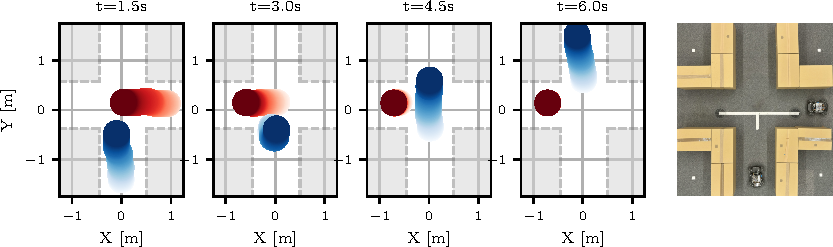
\includegraphics[width=\linewidth]{figures/mar25_1_tracer_graph.pdf}

    \caption{Demonstration of multi-agent collision avoidance, facilitated by my distributed SLAM system running locally on the Cambridge RoboMasters. Two robots are set 90° to each other in an intersection environment, with no direct view of the other robot and little visual overlap (right). The agent travelling along the Y axis is given a goal pose on the other side of the intersection, and successfully avoids a collision when the agent travelling along the X axis is pushed through the intersection. The trajectories generated by the SLAM system are presented on the left charts.}
    \label{fig:collision-avoidance}
\end{figure}

\begin{figure}[h]
    \centering
    \captionsetup{format=plain}
    \begin{minipage}[b]{0.62\linewidth}
        \centering
        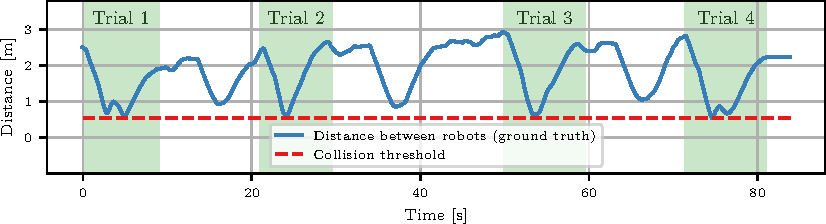
\includegraphics[width=\linewidth]{figures/mar25_1_distance_plot.pdf}

        \caption{Plot of ground truth distance between the two robots throughout all four collision avoidance trials conducted in the intersection environment. The dips between trials are the robots' positions being reset. \autoref{fig:collision-avoidance} visualizes Trial 4 in more detail.}
        \label{fig:collision-avoidance-distance-plot}
    \end{minipage}\hfill%
    ~
    \begin{minipage}[b]{0.34\linewidth}
        \centering
        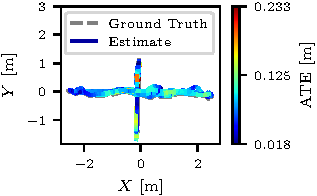
\includegraphics[width=\linewidth]{figures/mar25_1_trajectory.pdf}
        \caption{Collision avoidance estimated trajectory and ground truth. The RMS ATE is 0.074 meters.}
        \label{fig:tum-traj}
    \end{minipage}
\end{figure}

My projected included the development of an augmented reality visualization system to view my SLAM system's data overlayed on top of a video captured by an external camera. \autoref{TODO} shows a snapshot of this visualization, with the agents' map points and predicted locations overlayed on top of a video.